\section{Project Structure}

\par We plan to achieve such a mechanism by implementing and bridging the following six components:

\begin{figure}
  \centering
    \makebox[\textwidth]{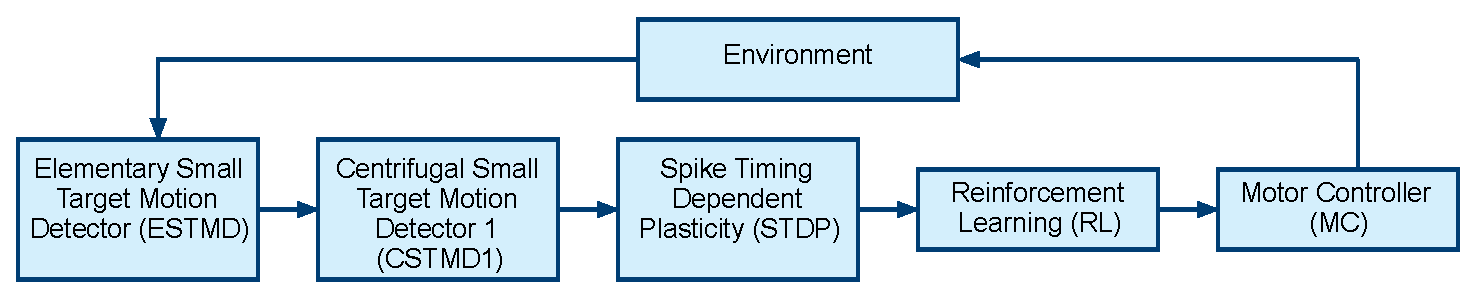
\includegraphics[width=\textwidth]{Project_Structure.eps}}
  \caption{Simulation pipeline}
  \label{modules}
\end{figure}


 \par \textbf{ESTMD}: A series of frames will be passed as input to an \textbf{Elementary Small Target Motion Detector}, which will identify and isolate small moving targets from a noisy background\cite{ESTMD1} and generate neural spikes\cite{ESTMD2}, and then pass the information\cite{ESTMD3} on to the CSTMD1.
 \par \textbf{CSTMD1}: The \textbf{Centrifugal Small Target Motion Detector 1} is the core of the project, implemented as a multicompartmental bistable neuron model\cite{CSTMD1}, which will choose a single target and ignore others. Depending on the input, the neuron will fire a specific repeatable pattern of spikes which will be passed to the STPD. The model will utilise reconstructed morphology based off previous academic research  \cite{Geurten3277}.
 \par \textbf{STDP} The \textbf{Spike Timing Dependent Plasticity} mechanism will learn how to recognise patterns \cite{stdp1}\cite{stdp2} in the output of the CSTMD1 and parse them into distinct signals for the action selection components (RL and MC).
 \par \textbf{RL}: The \textbf{Reinforcement Learning} component use a neural network to associate the recognised patterns \cite{IZ1} it has received with a set of possible actions by the Motor Controller. After the action has been performed, it will then alter the neural network weightings based upon the effectiveness of the action.
\par \textbf{MC}: The \textbf{Motor Controller} will perform an action selected by the RL on the dragonfly's state within the environment.
\par \textbf{Environment}: This will keep track of the position of the predator and will generate moving prey. It will construct frames for the predator's view which will be passed to the ESTMD. Ultimately we aspire to replace this module with a camera mounted drone.
  